\documentclass{article}
\usepackage[utf8]{inputenc}
\usepackage{hyperref}
\usepackage{graphicx}
\usepackage{subcaption}
\usepackage{cite}
\usepackage{float}
\usepackage{etoc}
\usepackage{blindtext}
\usepackage{amsmath}
\usepackage{amssymb}


%quote
\usepackage{epigraph}
\setlength\epigraphwidth{0.505\textwidth}
\setlength\epigraphrule{0pt}

% margins
\usepackage[a4paper, total={6in, 10in}]{geometry}

% spacing
\setlength{\parindent}{0em}
\setlength{\parskip}{1em}

% fonts (the same as NIPS 2016)
\renewcommand{\rmdefault}{ptm}
\renewcommand{\sfdefault}{phv}

\title{Interferenční mechanizmus\vspace{-1em}}
\author{Tomáš Vlk (vlktoma5@fit.cvut.cz)}
\date{\today}

\begin{document}

\maketitle

\section*{Úvod}

Interferenční\footnote{Občas nazývaný jako vyvozovací} mechanizmus tvoří jádro znalostního systému. Existuje více metod jak udělat interferenční mechanismus, ty jsou:

\begin{itemize}
\item \textbf{Logické metody}
\item \textbf{Zpětné nebo přímé zřetězení}
\item \textbf{Generování a testování}
\item \textbf{Využití analogií}
\end{itemize}

\section*{Logické metody}

Dedukce, abdukce a indukce vycházejí z výrokové logiky. Provedeme převod znalostí do exaktní matematické podoby v predikátové logice. Následně vyvozujeme závěry ze souboru pravidel. Lze použít například program OTTER nebo Prover9.

\begin{figure}[h]
\begin{center}
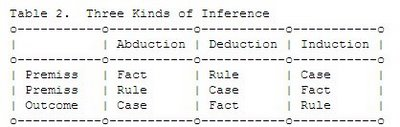
\includegraphics[scale=0.7]{TKI.jpg}
\caption{Logické metody}
\end{center}
\end{figure}

\subsection*{Dedukce}

Platí pravidlo a platí předpoklad. Odvozujeme platnost závěru\footnote{Modus ponens}. Tedy $A, A \Rightarrow B | B$. Alternativně platí pravidlo a neplatí závěr. Odvozujeme tedy neplatnost předpokladu\footnote{Modus tollens}. Neboli $\neg B, A \Rightarrow B | \neg A$. Příkladem je například "Jestliže prší, je mokro. Není mokro, tedy neprší".\par

Jestliže nemůže součastně platit A a B a platí A, nemůže platit B.\footnote{modus ponendo tollens} Neboli $\neg (A \wedge B) \wedge A \Rightarrow \neg B$. Příkladem může být "Není pravda, že pojedu autem a zároveň autobusem. Pojedu autem. Z toho vyplývá, že nepojedu autobusem".

\subsection*{Abdukce}

Platí pravidlo a platí závěr. Předpoklad může a nemusí být pravdivý. Domníváme se, že předpoklad může platit. Neboli $B, A \Rightarrow B | A$.

\subsection*{Indukce}

Opakované pozorování, že se A a B vyskytují součastně, odvozujeme tedy, že mezi A a B je vztah implikace. Neboli $A \Rightarrow B$ nebo $B \Rightarrow A$.

\section*{Zpětné zřetězení}

Používané zejména pro diagnostické znalostní systémy. Vycházíme z cílů a snažíme se najít pravidla která danný cíl potvrdí nebo vyvrátí. Vracíme se tedy zpětně od cílu k dotazům, s použitím dedukce. Pravidla lze vyhodnocovat více způsoby, mohou mít například přidělené priority.\par

Výhodami zpětného zřetězení je účinnost při malém množství hypotéz a hledání pouze fakt potřebných pro splnění cíle. Na druhou stranu postupuje splepě od cíle a má problém při velkém množství hypotéz a malém množství vstupních dat.

\section*{Přímé zřetězení}

Využívané zejména pro generativní znalostní systémy. Z předpokladů se snažíme vyvodit závěry, bez znalosti cílů. Opak zpětného zřetězení. Vzhledem k principu jakým přímé zřetězení probíhá je velmi náchylné na pořadí ve kterém vyhodnocuje pravidla.\par

Mezi výhody přímeho zřetězení patří schopnost generovat z malého množství informací velké množství nových faktů, díky tomu se výborně hodí pro plánování. Na druhou stranu není schopen rozlišit důležitost informace a prostě generuje vše, taktéž není možné zaručit pořadí kladení otázek a tudíž může být jejich pokládání nelogické.

\begin{figure}[h]
\begin{center}
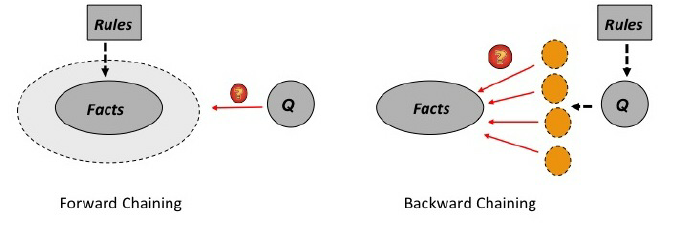
\includegraphics[scale=0.5]{FBC.png}
\caption{Přímé vs zpětné zřetězení}
\end{center}
\end{figure}

\section*{Generování a testování}

Opakovaně generujeme možná řešení a testujeme, zda vyhovují všem požadavkům. Většinou se používá pro generativní znalostní systémy. Znalosti jsou reprezentovány IF-THEN pravidly. Pokud exituje objekt, který vyhovuje podmínkám pravidla nazveme to nasycením předpokladů. Dvojice pravidla a jeho nasycení se nazývá instancí.

\section*{Analogie}

Analogie je postavená na hledání podobných již vyřešených případů. Databáze znalostí je tedy tvořena pouze souborem již vyřešených případů. Je jednodušší tento systém vytvořit, protože je snazší zajistit pro něj potřebné znalosti, ale je nutné zajistit metriku k porovnání s případy, které už máme v databázi znalostí.

\section*{Fungování znalostního systému}

Běh ZS má tři hlavní fáze:

\begin{itemize}
\item \textbf{Porovnání}\footnote{Angl. match} - vytvoření rozhodovací množiny, která obsahuje všechna v dané chvíli aplikovatelná pravidla

\item \textbf{Rozhodnutí sporu}\footnote{Angl. conflict resolution} - výběr právě jedné instance z rozhodovací množiny

\item \textbf{Úkon}\footnote{Angl. act} - provedení akcí pravé strany vybrané instance. Důsledkem může být přidání nebo odstranění předpokladu z množiny možných předpokladů, přidání pravidla do báze znalostí apod.
\end{itemize}

\subsection*{Strategie řešení konfliktu}
	
Existují různé strategie řešení konfliktu, jako třeba:

\begin{itemize}

\item \textbf{Prohledávání do hloubky}\footnote{Angl. depth strategy} - Preferují se pravidla používající aktuálnější data

\item \textbf{Prohledávání do šířky}\footnote{Angl. breath strategy} - Preferují se pravidla používající starší data

\item \textbf{Strategie složitosti}\footnote{Angl. complexity strategy} - Preferována jsou speciálnější pravidla

\item \textbf{Strategie jednoduchosti}\footnote{Angl. simplicity strategy} - Preferována jsou jednodušší pravidla

\end{itemize}

\end{document}
